\documentclass[a4paper]{article}

\usepackage[utf8]{inputenc}   % LaTeX, comprends les accents !
\usepackage[T1]{fontenc}      % Police contenant les caractères français
\usepackage[french]{babel}  
% \usepackage{fullpage}
% \usepackage{graphicx}
% \usepackage{wrapfig}
% \usepackage{float}
% \usepackage{blindtext}
\usepackage[colorlinks=true,linkcolor=black,urlcolor=black,bookmarksopen=true,bookmarksnumbered=true]{hyperref}
\usepackage{bookmark}
\usepackage{listings} % pour inclure du code
\usepackage{mathtools} % équation mathématique

% \graphicspath{ {./img/} }
\begin{document}
	\title{Évaluation expérimental de Choco-solver\\librairie de programmation par contraintes}
	\author{\emph{Paul Fontaine - Tony Nguyen}\\
  M1 informatique Algorithme - M1 informatique Génie Logiciel\\
	Faculté des Sciences\\
	Université de Montpellier}
	\date{\today}
	\maketitle
	\thispagestyle{empty}
	% \begin{figure}[h]
	% 	\includegraphics[scale=.1]{selfie_tony_clementine.jpg}
	% 	% \includegraphics[width=\textwidth]{recon.png}
	% 	\centering
	% \end{figure}
	\newpage
	\thispagestyle{empty}
	\tableofcontents
	\newpage
	% \thispagestyle{empty}
	% \listoffigures
	\newpage
  \section{Identification de la transition de phase} 
  \subsection{Génération des benchmark}
  \paragraph{}
    Tout d'abord, avec un script fournis (voir Listing \ref{test}) et personalisé, nous avons générer un jeux d'essais(=benchmark) pour des Constraint Satisfaction Problem (CSP) de paramètre <2,35,17,249,t>.\\
    \emph{l'arité des contraintes k=2\\
    le nombre de variables n=35\\
    la taille du plus grand des domaines=17\\
    le nombre de contraintes e=249\\
    la dureté t=[29.4;35.6] avec un nombre de tuples par contraintes (la variable i dans le script) compris entre 186 et 204\\
    La densité est TODO}
  \lstinputlisting[language=Octave, caption=Script de génération des jeux d'essais test \label{test}]{generateurBench.sh}
  \paragraph{Remarque}
    Nous avons des contraintes binaires. Toutes les variables ont des domaine de taille égaux.
  \paragraph{}
    Dans notre benchmark, nous avons donc 10 niveau de dureté avec 30 CSP par niveau.
  \subsection{Méthode}
  \paragraph{}
    Pour chaque CSP, \emph{nous allons cherché une solution pendant 30 secondes}, si choco solver trouve une solution avant, on associe cette événement à une \textbf{réussite}. Si choco a exploré tout l'arbre de recherche avec le temps impartie, c'est un \textbf{échec}. Si choco solver ne parviens ni a trouver une solution ni a exploré tout l'arbre avec le temps maximal, alors nous alors dire que c'est un \textbf{Time Out}.
  \subsection{Calcul}
  \paragraph{}
    Soit la fonction $g_a^b$ : (a correspond à un CSP dans notre benchmark et b un niveau de dureté)\\
    \[ g_a^b() =
      \begin{cases}
        1       & \quad \text{si solution trouvé}\\
        0       & \quad \text{si Time Out}\\
        0       & \quad \text{si pas de solution}\\
      \end{cases}
    \]
  \paragraph{}
    Soit f(x) la fonction qui calcule le pourcentage de réussite en fonction du niveau de dureté x de la façon suivante:\\
    \begin{center}
      $f(x)=\cfrac{\displaystyle\sum_{k=1}^{30} g_k^x()}{30}$
    \end{center}
  \newpage
  \subsection{Résultat}
  \paragraph{}
    Nous pouvons observé sur la figure \ref{fig:graphTransi}, une transition de phase entre 30 et 34 pourcent.
  \paragraph{}
    Nous pouvons en conclure que \textbf{les CSP difficile à résoudre ont une densité autour de 32 pourcent}. Cette information nous sera utile pour la suite...
  \begin{figure}
				\centering
				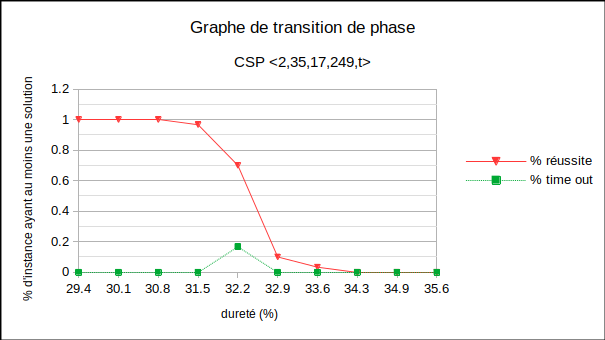
\includegraphics[width=1.0\textwidth]{graphTransition.png}
				\caption{Graphe de f(x)}
				\label{fig:graphTransi}
	\end{figure}
\end{document}